\documentclass[9pt,twocolumn,twoside]{../../styles/osajnl}
\usepackage{fancyvrb}
\journal{i524} 

\title{ASKALON}

\author[1,*]{Abhishek Naik}

\affil[1]{School of Informatics and Computing, Bloomington, IN 47408, U.S.A.}
\affil[*]{Corresponding authors: ahnaik@indiana.edu}

\dates{project-002, \today}

\ociscodes{Cloud, I524}

% replace this with your url in github/gitlab
\doi{\url{https://github.com/cloudmesh/sp17-i524/blob/master/paper2/S17-IR-2022/report.pdf}}


\begin{abstract}
ASKALON is a Grid application development and computing environment
which aims to provide a Grid to the application developers in an
invisible format \cite{Workflow-book}.  This will simplify the
development and execution of various workflow applications on the
Grid.  This will not only allow a transparent Grid access but also
will allow the high-level composition of workflow applications.
ASKALON basically makes use of five services: Resource Manager,
Scheduler, Execution Engine, Performance Analysis and Performance
Prediction \cite{RMBDP-Book}.\newline
\end{abstract}

\setboolean{displaycopyright}{true}

\begin{document}

\maketitle

\section{Introduction}

A Grid is basically a combination of hardware and software that
provides reliable and pervasive computation abilities.  Grid based
development methodologies are used for application development.  These
Grid-based development methodologies emphasize providing the
application developer with a non-transparent grid.  ASKALON provides
such invisible grid to the application developers.  While using
ASKALON, the Grid work flow applications are made using Unified
Modeling Language (UML) based services \cite{Workflow-book}.  Besides
this, it also enables integration of the workflows that have been
created programmatically using languages such as XML.  ASKALON
typically requires some middleware for this.

\section{Description}

When using ASKALON, the users need to create Grid workflow
applications at a higher level of abstraction using the Abstract Grid
Workflow Language (AGWL) which is based on XML.  This representation
of the workflow is later passed on to the middleware layer for
scheduling and exection.  Figure 1 shows the typical architecture of
ASKALON.

\begin{figure}[htbp]
  \centering
  \fbox{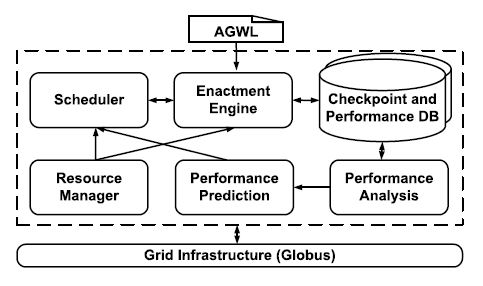
\includegraphics[width=\linewidth]{images/ASKALONArchitecture}}
  \caption{ASKALON Architecture \cite{Workflow-book}}
\end{figure}

As shown in the figure, the major service components are the
Resource Manager which is used for management of the various
resources, the Scheduler that is used for scheduling the various
workflow applications onto the Grid, the Execution engine which
provides reliable and fault tolerant execution, the Performance
  analyser that analyses the performance and detects bottlenecks and
the Performance predictor that estimates the execution times.
The following paragraphs provide a brief description about these
services:

\subsection{Resource Manager}
The Resource Manager service is responsible for the management of
the resources like the procurement, allocation, reservation and
automatic deployment.  It usually works hand in hand with the AGWL.
In addition to this management of resources, the main task of the
Resource manager is to abstract the users from low-level Grid
middleware technology.

\subsection{Scheduler}
The Scheduler service is responsible for the scheduling (or
mapping) of various workflow applications onto the Grid using
optimization algorithms and heuristics based on graphs.  In addition
to this, it monitors the dynamism of the Grid infrastructures thorough
an execution contract and adjusts the optimised static schedules
accordingly.  The Scheduler thus provides Quality of Service (QoS)
dynamically.  It usually uses one out of the three algorithms -
Heterogeneous Earliest Finish Time (HEFT), Genetic or Myopic.  HEFT
algorithm schedules the various workflows by creating an ordered lists
of tasks and then mapping the tasks onto the resources in the most
efficient way.  Genetic algorithms are inspired by Darwin's theory of
evolution and work using its the princples of evolution while the
Myopic algorithms are basically just-in-time approaches, since they
make greedy decisions that would be best in the current scenario.

\subsection{Execution Engine}
The Execution Engine service also known as the Enactment
  Engine service performs tasks such as checkpointing, retry,
restart, migration and replication.  It thus aims to provide reliable
and fault tolerant execution of the workflows.

\subsection{Performance Analyser}
The Performance Analyser service provides support to the
automatic instrumentation and bottleneck detection within the Grid
workflow executions.  For example, excessive synchronization, load
imbalance or non-scalability of the resources might result in a
bottleneck and it is the responsibility of the Performance Analyser to
detect and report it.

\subsection{Performance Prediction}
The Performance Prediction services predicts the performance,
i.e., it emphasises on the execution time of the workflow activities.
It uses the training phase and statistical methods for this.

\section{Workflow Generation}
ASKALON basically offers two interfaces: graphical model based on UML
and a programmatic XML based model \cite{Workflow-book}.  The main aim
of both these interfaces is to generate large-scale workflows in a
compact as well as intuitive form:

\subsection{UML-modeling based}
ASKALON allows creation of workflows via a modeling service similar to
UML diagrams.  This service combines Activity Diagrams and works in a
hierarchical fashion.  This service can be implemented in a platform
independent way using the Model-View Controller (MVC) paradigm.  This
service can then be shown to contain three parts: a Graphical User
Interface (GUI), model traverser and model checker.  This GUI in turn
comprises of the menu, toolbar, drawing space, model tree and the
properties of the elements.  The drawing space can contain several
diagrams.  The model traverser, as the name suggests, provides a way
to move throughout the model visiting each element and accessing its
properties.  The model checker on the other hand is responsible for
the correctness of the model.

\subsection{XML-based Abstract Grid Workflow Language}
The Abstract Grid Workflow Language enables the combination of various
atomic units of work called as activities.  These activities are
interconnected through control-flow and data-flow dependencies.
Activities can in turn be of two levels: activity types and activity
deployments.  An activity type describes the semantics or functions of
an activity, whereas the activity deployment points to a deployed Web
Service or executable.  AGWL is not bounded to any implementation
technologies such as the Web Services.  Also, the AGWL representation
of a typical workflow can be generated in two ways: automatically via
the UML representation or manually by the user.  In both the cases,
AGWL serves as the input to the ASKALON runtime middleware services.

\section{Comparison with other counterparts}
Few experiments have been carried out using the seven Grid clusters of
the Austrian Grid \cite{Austrian-grid} and a group of 116 CPUs.
Figure 2 represents performance of the individual clusters, wherein
each cluster aggregates the execution time of all the workflows
executed on a single CPU.  As can be inferred from the figure, the
fastest cluster is around thrice faster than the slowest one.

DAGMan \cite{DAGMan} is a scheduler that is used for Condor jobs that
have been organized in the form of a Directed Acyclic Graph (DAG).
Scheduling doesn't use any specialized optimization techniques and is
done simply using matchmaking.  Fault tolerance is done using rescue
DAG that is automatically generated whenever some activity fails.  As
against this, the ASKALON checkpointing also takes care of the fact
when the Execution Engine itself fails.  Thus, the checkpointing
provided by ASKALON is more robust compared to that by other
counterparts like DAGMan.

ASKALON differs in many respects compared to other projects like
Gridbus \cite{Gridbus} and UNICORE \cite{Unicore}.  In ASKALON, the
AGWL allows a scalable specification of many parallel activities by
using compact parallel loops.  The Enactment Engine also enables
handling of very large data collections that are generated by
large-scale controls and data-flows.  The HEFT and genetic search
algorithms that the ASKALON scheduler implements, are not used by the
other projects, like the ones mentioned above.  The Enactment Engine
also provides checkpointing of workflows at two leves for restoring
and resuming, in case the engine itself fails.  In ASKALON, a lot of
emphasis is laid on the clear separation between the Scheduler and the
Resource Manager.  It thus proposes a novel architecture in terms of
physical and logical resources and thus provides brokerage,
reservations and activity type to deployment mappings.

\begin{figure}[htbp]
  \centering
  \fbox{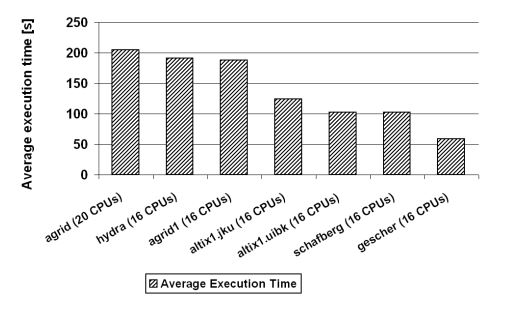
\includegraphics[width=\linewidth]{images/AustrianGrid}}
  \caption{Performance of Austrian Grid clusters \cite{Austrian-grid}}
\end{figure}

\section{ASKALON in Big Data projects}
ASKALON has been used in the design of Meteorological Stimulations in
the Cloud \cite{ASKALON-Big-data-project}.  In order to deploy the
application on a distributed Grid infrastructure, the simulation code
was split into a workflow called the RainCloud, which was represented
using ASKALON.  Figure 3 denotes the graphical representation of this
workflow.

\begin{figure}[htbp]
  \centering
  \fbox{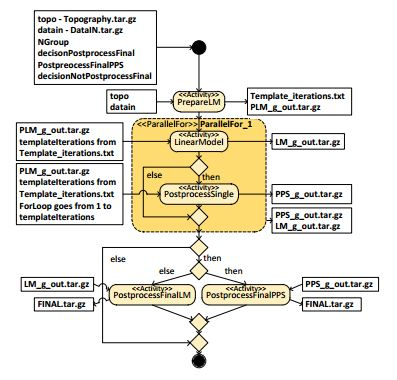
\includegraphics[width=\linewidth]{images/Meteorological-workflow}}
  \caption{Graphical representation of the Meteorological workflow \cite{ASKALON-Big-data-project}}
\end{figure}

This workflow was flexible in the sense that it could be easy extended
to suite the needs of some other projects.  For example, this workflow
setup was extended for an investigation of precipitation/snow
accumulation on the Kongsvegen glacier on Svalbard, Norway, as a part
of the SvalClac project \cite{ASKALON-Big-data-project}.

\section{Conclusion}

ASKALON supports workflow integration using UML and also provides an
XML based programming interface.  This effectively abstracts the end
user from the low level middleware technologies.  The Resource Manager
handles the logical and physical resources and the workflow activities
to provide features such as authorization, Grid resource discovery,
selection, allocation and interaction.  Scheduler makes use of some
algorithms like HEFT or other genetic algorithms which deliver high
performance.  It highly benefits from the Performance Prediction
service which in turn depend upon the training phase and the
statistical methods used.  The Execution Engine handles data
dependencies and also working on high volume data - something that is
highly useful in Big Data related applications and projects.  The
Performance Analyser analysis the performance benchmarks.  Typically,
the overhead of ASKALON middleware services which consist of the
Resource Manager, Scheduler and Performance prediction are usually
constant, thereby requiring less execution time holistically.

Thus, to conclude, we focused on ASKALON as a Grid application
development environment.  We also saw the various architectural
components of ASKALON as well as the comparisons amongst the different
Grid clusters that were used.  We also saw some Big Data use cases
wherein ASKALON was used and the flexibility with which the workflow
setup using ASKALON was extended to support different projects.

% Bibliography

\bibliography{references}

\end{document}
